% !TEX root = report.tex

\section{Results}\label{sec:results}

The 12 generated datasets, as described in \autoref{sec:model}, are:
%As a summary of the 12 generated datasets, they are:
\begin{itemize}
    \item w.r.t. two reference frames (sensor and body)
    \item with and without normalization
    \item optionally augmented manually or with ADASYN
\end{itemize}
The results are explained in a top-down fashion to progressively prune out combinations.
Subsequent considerations still apply to previously excluded parts.
The complete set of results can be generated using the notebooks.
Note that for Keras models and scikit-learn's SGD implementations accuracy equals weighted recall, so we will use this as comparison metric.

%We want to put evidence in the fact that performance differences in some cases are minimal and can be linked either to the stochastic nature of the methods and to the fact that our models perform very well on the most represented classes (around 98/100\%).
%The complete set of results can be generated using the publicly available companion notebook.

\subsection{Reference frame}
Comparing the same networks, trained over the same type of dataset, we can note how performance are superior with sensor-referenced data, instead of using data referenced to the body frame, and it is easy to see how even plain global accuracy is lower on such datasets, an example is in \tab{tab:body_sensor}.
This is a surprising aspect because the coordinate transformation should act as a stabilizer to equalize measurements and generalize them as noted in~\cite{Liano-HMM}.

\begin{table}[ht]
\centering
\caption{Best accuracy value (\%) on some datasets, body (\texttt{B*}) and sensor (\texttt{S*}) reference frame. \textit{Mixed} is CNN-LSTM, due to space constraints.}
\label{tab:body_sensor}
\begin{tabular}{lrrrrr}
\toprule
net &  Conv1D-2C1D-do0.3 &  Conv2D-Ha &  TwoLSTM &  TwoGRU &  CNN-LSTM \\
ds   &                    &            &          &         &           \\
\midrule
BADA &             98.062 &     95.528 &   98.085 &  98.085 &    98.447 \\
BNOR &             97.933 &     95.166 &   98.120 &  98.143 &    98.435 \\
SADA &             99.194 &     97.898 &   99.194 &  99.159 &    99.451 \\
SNOR &             99.159 &     98.073 &   99.159 &  99.113 &    99.358 \\
\bottomrule
\end{tabular}

\end{table}

\subsection{Normalization}
As common practice suggest we performed normalization on datasets using training set's mean and standard deviation.
In general, by looking at global accuracy, there is no strict rule to say that using it is better than leaving data as is.
The results are so near that could even be linked to stochasticity of trainings and to highly imbalanced classes.
From \tab{tab:norm-aug} we can note how there are cases like CNN-LSTM and SADA(n) where normalized dataset goes better, and cases like TwoGRU and SAHC(n) where it is the opposite.
So we cannot come up with a definitive answer for this normalization question.

\begin{table}[ht]
\centering
\caption{Best accuracy value (\%) for sensor-referenced datasets: ADASYN-augmented (\texttt{SADA}), manually augmented (\texttt{SAHC}), normalized but not augmented (\texttt{SFRA}). Not normalized versions of these three datasets are \texttt{SADAn}, \texttt{SAHCn} and \texttt{SFRAn}.}
\label{tab:norm-aug}
\begin{tabular}{c|ccccc}\toprule
Dataset & Conv1D            & Conv2D            & 2LSTM             &  2GRU             & Mixed \\\midrule
SADA    & \textbf{99.194}   & 97.898            & 99.194            & 99.159            & \textbf{99.451} \\
SADAn   & 99.066            & 98.003            & \textbf{99.241}   & \textbf{99.288}   & 99.183 \\
SAHC    & 97.957            & \textbf{98.284}   & 99.206            & 97.840            & 99.416 \\
SAHCn   & 99.043            & 98.260            & 99.229            & 99.253            & 99.183 \\
SFRA    & 99.159            & 98.073            & 99.159            & 99.113            & 99.358 \\
SFRAn   & 98.984            & 98.272            & 98.564            & 99.206            & 99.113 \\\bottomrule
\end{tabular}
\end{table}

% not related here but goes to next page
\begin{table*}[ht]
\centering
\caption{Saving epoch, per-class accuracy, global accuracy, weighted and standard precision and recall (\%), for the two most prominent models.
Each value is reported according to the four metrics presented in section~\ref{ssec:metrics} (top to bottom, same order).}
\label{tab:metrics}
\begin{tabular}{lc|ccccccc|cccc}\toprule
Model & E &\labelbox{label-running} & \labelbox{label-walking} & \labelbox{label-jumping} & \labelbox{label-standing} & \labelbox{label-sitting} & \labelbox{label-lying} & \labelbox{label-falling} & Acc. & W Prec. & Prec. & Recall \\\midrule
\multirow{2}{*}{2GRU}     & 101 & 100.000 & 99.014 & 93.897 & 99.588 & 99.637 & 99.874 & 87.273 & 99.288 & 99.284 & 99.293 & 99.282 \\
                          &  84 & 100.000 & 99.113 & 90.141 & 99.706 & 99.577 & 99.748 & 90.909 & 99.264 & 99.262 & 99.293 & 99.247 \\
\multirow{2}{*}{(SADAn)}  & 101 & 100.000 & 99.014 & 93.897 & 99.588 & 99.637 & 99.874 & 87.273 & 99.288 & 99.284 & 99.293 & 99.282 \\
                          &  84 & 100.000 & 99.113 & 90.141 & 99.706 & 99.577 & 99.748 & 90.909 & 99.264 & 99.262 & 99.293 & 99.247 \\\midrule
\multirow{2}{*}{Mixed}    &  27 & 100.000 & 99.211 & 92.488 & 99.794 & 99.758 & 99.874 & 94.545 & 99.451 & 99.454 & 99.464 & 99.452 \\
                          &  21 & 100.000 & 99.113 & 92.488 & 99.676 & 99.819 & 99.874 & 92.727 & 99.381 & 99.382 & 99.394 & 99.382 \\
\multirow{2}{*}{(SADA)}   &  27 & 100.000 & 99.211 & 92.488 & 99.794 & 99.758 & 99.874 & 94.545 & 99.451 & 99.454 & 99.464 & 99.452 \\
                          &  21 & 100.000 & 99.113 & 92.488 & 99.676 & 99.819 & 99.874 & 92.727 & 99.381 & 99.382 & 99.394 & 99.382 \\\bottomrule
\end{tabular}

\end{table*}

\subsection{Augmentation}
Evaluation is problematic also in this section: from \tab{tab:norm-aug} we can note how augmented datasets do not \textit{always} perform better than non-augmented ones.
What is noted instead is that \textit{at least} one of the two augmented versions performs better than ``plain'' ones.
%
%\comment{As can be seen in \tab{tab:norm-aug}, also here w.r.t. augmentation there are a bit of problems since augmented datasets do not \textit{always} perform better than not augmented ones.
%What we can surely see instead is that \textit{at least} one of the two augmented versions performs better than plain ones.
%Moreover ADASYN augmentation achieve better results wrt manual one in all networks but Conv2, taking in consideration both normalized and not normalized versions of the ds.}
%\comment{This behaviour could was expected because augmentation is performed to enhance less represented classes and as such they do not have great influence on a global metric. A proof of that can be seen in \fig{fig:cm-sahc-conv2d} and \fig{fig:cm-snor-conv2d} where is clear that \textit{jumping} and \textit{falling} reaches way better per-class accuracies.}
This behavior was expected, because augmentation is performed to enhance less represented classes and as such they do not have great influence on a global metric.
A proof can be seen in \fig{fig:cm-sahc-conv2d} and \fig{fig:cm-snor-conv2d} where clearly \textit{jumping} and \textit{falling} reaches way better per-class accuracies.
Moreover, ADASYN achieve better results w.r.t. manual augmentation in all networks but Conv2D, considering both normalized and non-normalized versions.
This also proves augmentation is useful and worth.
Paired with previous results, here are the best models overall: TwoGRU over SADAn, CNN-LSTM over SADA.

\begin{figure}[ht]
\hspace*{+0.15cm}
    \centering
    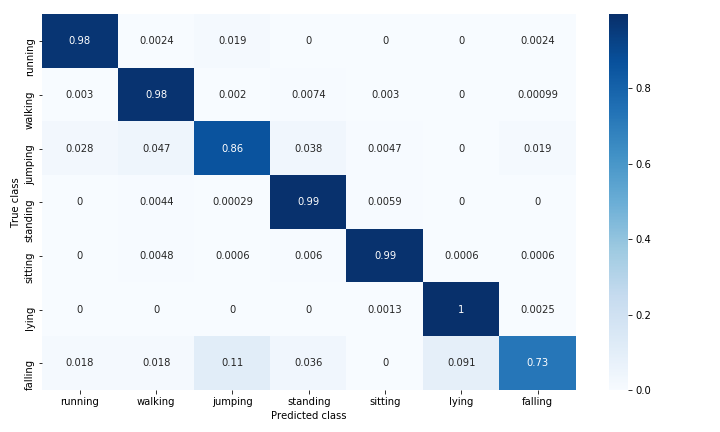
\includegraphics[width=1.05\columnwidth]{images/plot-cm-SAHC_Conv2D.png}
    \caption{Confusion matrix of Conv2D model, SAHC dataset.}
    \label{fig:cm-sahc-conv2d}
\end{figure}

\begin{figure}[ht]
\hspace*{+0.15cm}
    \centering
    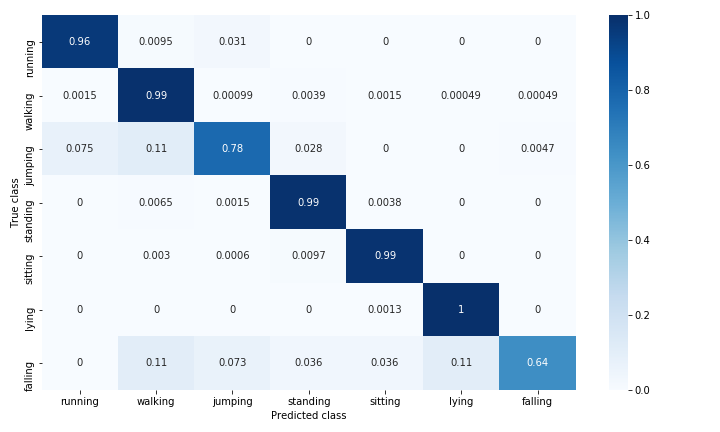
\includegraphics[width=1.05\columnwidth]{images/plot-cm-SNOR_Conv2D.png}
    \caption{Confusion matrix of Conv2D model, SFRA dataset.}% because snor == sfra and sfra == sfran
    \label{fig:cm-snor-conv2d}
\end{figure}

\subsection{Models and metrics}

By looking at \tab{tab:metrics}, we notice how:
\begin{itemize}
\begin{samepage}
    \item defined metrics may couple together: this happens when the model is saved at the same epoch according to two different metrics. Most of the times $\mathrm{A}$ couples with $\mathrm{APR}$ while $\mathrm{AoL}$ couples with $\mathrm{APRoL}$, but there may be exceptions like CNN-LSTM on SAHCn, where $\mathrm{A}$ differs from $\mathrm{APR}$.
    \item generally, accuracy $\mathrm{A}$ (weighted recall) gives best results.
    \item the best model is CNN-LSTM.
\end{samepage}
\end{itemize}

In general, our models achieve high accuracy within a small number of epochs ranging from a few to a hundred or so.
2D CNN and CNN-LSTM exhibit slight overfitting (see \fig{fig:acc-loss-sada-mixed}), that could be tackled with additional regularization or learning rate's decay.
Anyway, models are saved before this happens.

\begin{figure}[ht]
    \centering
    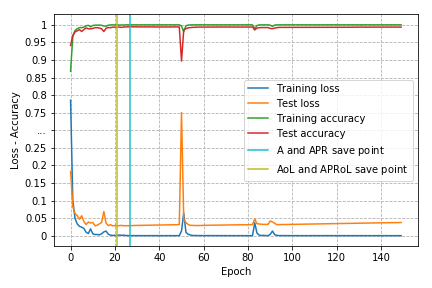
\includegraphics[width=\columnwidth]{images/plot-acc-loss-SADA_CNN-LSTM.png}
    \caption{CNN-LSTM, SADA dataset: training accuracy and loss.}
    \label{fig:acc-loss-sada-mixed}
\end{figure}

Only comparing the two best models in \tab{tab:norm-aug}, CNN-LSTM performs slightly better, even if the 0.163\% gained (from 99.288\% to 99.451\%) is a stunning 22.9\% of the remaining available accuracy.
Taking the maximum and minimum values, we span from 97.840\% to 99.451\%, covering about 74.6\% of the remaining achievable accuracy.

\begin{table*}
\centering
\caption{Comparison between our best networks and datasets combination and original results from \cite{FrankNadales} based on Dynamic Bayesian Networks: precision (first) and recall (second) values for each class. Best results in bold (virtually rounded).}
\label{tab:soa}
%\begin{tabular}{l|cllllllllllllll}\toprule
%& \multicolumn{2}{c}{\textbf{RUNNING}} & \multicolumn{2}{c}{WALKING} & \multicolumn{2}{c}{\textbf{JUMPING}} & \multicolumn{2}{c}{STANDING} & \multicolumn{2}{c}{SITTING} & \multicolumn{2}{c}{\textbf{LYING}} & \multicolumn{2}{c}{\textbf{FALLING}} \\ \midrule
%
%\begin{tabular}{l|ccccccc}\toprule
%Model  & \labelbox{label-running} & \labelbox{label-walking} & \labelbox{label-jumping} & \labelbox{label-standing} & \labelbox{label-sitting} & \labelbox{label-lying} & \labelbox{label-falling} \\\midrule
%Conv1D & 97.912~~99.764       & \textbf{98.869}~~99.113 & \textbf{98.990}~~92.019          & 99.325~~\textbf{99.647}          & \textbf{99.879}~~99.698 & 99.369~~\textbf{99.369}       & \textbf{89.796}~~80 \\
%Conv2D & 96.948~~97.636       & \textbf{98.277}~~98.374 & 90.196~~86.385                   & 98.969~~\textbf{98.940}          & \textbf{98.315}~~98.731 & 99.246~~\textbf{99.622}       & 80~~72.727 \\
%2LSTM  & 98.601~~\textbf{100} & \textbf{99.407}~~99.162 & \textbf{98.030}~~\textbf{93.427} & 99.149~~\textbf{99.499}          & \textbf{99.697}~~99.517 & 99.873~~\textbf{99.369}       & \textbf{86.441}~~92.727 \\
%2GRU   & 99.063~~\textbf{100} & \textbf{99.259}~~99.014 & \textbf{95.694}~~\textbf{93.897} & 99.441~~\textbf{99.588}          & \textbf{99.517}~~99.637 & 99.497~~\textbf{99.874}       & \textbf{96}~~87.272 \\
%Mixed  & 97.465~~\textbf{100} & \textbf{99.407}~~99.211 & \textbf{98.995}~~92.488          & \textbf{99.559}~~\textbf{99.794} & \textbf{99.819}~~99.758 & \textbf{100}~~\textbf{99.874} & \textbf{92.857}~~94.545 \\
%DLR    & \textbf{100}~~93     & 98~~\textbf{100}        & 93~~93                           & \textbf{100}~~98                 & 97~~100                 & 100~~98                       & 80~~100 \\ \bottomrule
%\end{tabular}
%
\begin{tabular}{l|ccccccc}\toprule
Model  & \labelbox{label-running} running & \labelbox{label-walking} walking & \labelbox{label-jumping} jumping & \labelbox{label-standing} standing & \labelbox{label-sitting} sitting & \labelbox{label-lying} lying & \labelbox{label-falling} falling \\\midrule
Conv1D\footnotesize{-2C1D} & 97.91~~99.76 & \textbf{98.87}~~99.11 & \textbf{98.99}~~92.02 & 99.33~~\textbf{99.65}         & \textbf{99.88}~~99.70 & 99.37~~\textbf{99.37}        & \textbf{89.80}~~80.00 \\
Conv2D-Ha & 96.95~~97.64        & \textbf{98.28}~~98.37 & 90.20~~86.39                   & 98.97~~\textbf{98.94}          & \textbf{98.32}~~98.73 & 99.25~~\textbf{99.62}        & 80.00~~72.73 \\
TwoLSTM   & 98.60~~\textbf{100} & \textbf{99.41}~~99.16 & \textbf{98.03}~~\textbf{93.43} & 99.15~~\textbf{99.50}          & \textbf{99.70}~~99.52 & \textbf{99.87}~~\textbf{99.37}        & \textbf{86.44}~~92.73 \\
TwoGRU    & 99.06~~\textbf{100} & \textbf{99.26}~~99.01 & \textbf{95.69}~~\textbf{93.90} & 99.44~~\textbf{99.59}          & \textbf{99.52}~~99.64 & \textbf{99.50}~~\textbf{99.87}        & \textbf{96.00}~~87.27 \\
CNN-LSTM  & 97.47~~\textbf{100} & \textbf{99.41}~~99.21 & \textbf{98.99}~~92.49          & \textbf{99.56}~~\textbf{99.79} & \textbf{99.82}~~99.76 & \textbf{100}~~\textbf{99.87} & \textbf{92.86}~~94.55 \\
BN \cite{FrankNadales}  & \textbf{100}~~93    & 98~~\textbf{100}      & 93~~93                         & \textbf{100}~~98               & 97~~100               & 100~~98                      & 80~~100 \\ \bottomrule
\end{tabular}

\end{table*}

As per \tab{tab:soa}, comparing results with the work done in \cite{FrankNadales}, which is based on Dynamic unrestricted Bayesian Networks, we achieve better precision and recall in most of the classes, especially in the augmented ones, with almost all our best configurations.

Finally, in general TwoLSTM, TwoGRU and CNN-LSTM are the models that perform, regardless of normalization and augmentation, \textit{always} better than Conv2D-Ha and \textit{almost} constantly better than Conv1D-2C1D.

As for timings, we notice in \tab{tab:timings} that recurrent networks are much slower with respect to convolutional models, yielding only a low overall performance increase.
Notably, thanks to pooling and convolutional layers, the combined model actually achieves the best training speed overall, letting us conclude along with previous considerations that it is the best in our pool of analyzed networks.

\begin{table}[ht]
\centering
\caption{Mean sample processing time and epoch duration, \texttt{SAHC} dataset, 27611 samples. Benchmark on dual-core 2.30GHz CPU and NVIDIA\textregistered{} T4.}
% shape \texttt{(27611,128,9)}
\label{tab:timings}
\begin{tabular}{c|cccccc}\toprule
       & Conv1D & Conv2D  & 2LSTM & 2GRU  & Mixed \\\midrule
Sample & 235us  & 219us   & 3ms   & 2ms   & \textbf{175us} \\
Epoch  & 6.6s    & 6.0s   & 75s   & 53.8s & \textbf{4.8s}  \\\bottomrule
\end{tabular}
\end{table}

\subsection{Autoencoders}
Training of autoencoders is good and fast: as reported in \tab{tab:ae_train}, they reach 99\% accuracy on test set with a loss of 0.25 in less than five epochs.

\begin{table}[ht]
\centering
\caption{Accuracy and loss of trained AEs, for some datasets.}
\label{tab:ae_train}
\begin{tabular}{lrrrrrr}
\toprule
{} & \multicolumn{3}{l}{acc} & \multicolumn{3}{l}{loss} \\
net & CNN-LSTM-AE & CNN\_AE & LSTM-AE & CNN-LSTM-AE & CNN\_AE & LSTM-AE \\
ds   &             &        &         &             &        &         \\
\midrule
BAHC &       0.996 &  0.996 &   0.994 &       0.250 &  0.250 &   0.250 \\
BNOR &       0.993 &  0.994 &   0.993 &       0.812 &  0.812 &   0.812 \\
SADA &       0.997 &  0.996 &   0.955 &       0.581 &  0.581 &   0.586 \\
SAHC &       0.995 &  0.996 &   0.995 &       0.385 &  0.385 &   0.385 \\
SFRA &       0.998 &  0.986 &   0.986 &      12.099 & 12.101 &  12.101 \\
SNOR &       0.996 &  0.997 &   0.994 &       0.793 &  0.793 &   0.793 \\
\bottomrule
\end{tabular}

\end{table}

Instead, application of encoded data to the networks have not brought the expected improvements in any datasets or methods we used.
In general we noted comparable, and in some cases slightly lower, performance than the same networks trained on the original dataset. A few examples can be seen in \tab{tab:ae_comp}.

\begin{table}[ht]
\centering
\caption{Comparison between models trained on encoded data and on the original data.}
\label{tab:ae_comp}
\begin{tabular}{c|cccccc} \toprule
Model  & Dataset   & AE        & DS Acc. & AE Acc. \\\midrule
Conv1D & SAHC      & LSTM      & 99.416  & 98.751  \\
TwoGRU & BFRA      & CNN       & 98.085  & 96.298  \\
Mixed  & SADA      & CNN-LSTM  & 99.451  & 98.459  \\\bottomrule
\end{tabular}

\end{table}

Apart from being time costly to permute all of them, applications of SVM and LR in combination with L1, L2 and Elastic Net regularization terms do not provide good results: models tend to well learn long and stable activities, while being worse with \textit{running}, \textit{jumping} or \textit{falling} (see \fig{fig:cm-svm-sahc-mixed}).
We reached a top value of 90\% global test accuracy on a specific combination of AE and LR model.
Furthermore, there is no clear linking between performance and LR or SVM or with respect to regularization terms, which makes essential to loop all combinations to see the best one.

\begin{figure}
    \centering
    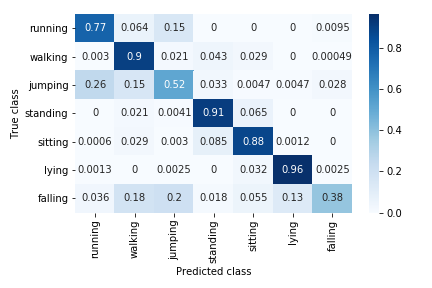
\includegraphics[width=\columnwidth]{images/plot-cm-SVM-L2-SAHC_Mixed.png}
    \caption{SVM with L2 regularization, CNN-LSTM encoding, SAHC dataset.}
    \label{fig:cm-svm-sahc-mixed}
\end{figure}

The pattern of results obtained over each dataset and network is in accordance with our previous findings: these methods cannot compete with the previously defined ones, and in our implementation it is better to process raw signals than to build methods on encoded features.
